% !TeX root = ../main.tex
\section{Background Literature Review}

To achieve these aims, a background literature review will be performed to ensure that the proposed methodology described later utilises best modern practices and research, and targets a clear gap in research. Focus will be placed on an overview of the problem, common approaches and prevalent models, and common model compression techniques. 

\subsection{Literature Review: Overview} As discussed in the introduction, modern sporting preparation and broadcast have put a larger emphasis on quantitative data than opinion-based analysis, especially with the rise of next-generation tracking and sensor technologies \cite{ReinMemmert2016}. Some of the most useful of these implementations explore tracking key statistics such as team pass completions percentages, possession, and team formation analysis through the use of object detection/tracking and pitch recognition \cite{zheng2025_review_football_cv,Mooney2014CVSports}. However, emphasis in this niche has been largely placed on accuracy over computational efficiency or real-time analysis, with some designed software systems requiring over 515B Floating Point Operations Per Second (FLOPS) \cite{roboflow_sports_repo}, which edge devices cannot maintain.

\subsection{Literature Review: Common Approaches} Modern computer vision-based approaches to estimating possession and formation often utilise object detection models coupled with object tracking algorithms to produce Multiple Object Tracking (MOT) outputs \cite{tracking}. This allows identities (in the form of bounding boxes) for on-screen outfield players, goalkeepers, referees, and the ball to be used for statistic generation. From here, clustering techniques such as K-means and mean shift methods are often applied, separating detecting players into two teams, as well as determining the goal-keepers \cite{ZhengLiu2012ColorRecognition}. This team assignment allows detailed estimates of possession and pass completion to be determined. 

Alongside object detection for players, a variety of different key-point detection strategies are often used to detect the location on screen of relevant pitch markings, such as the corners, penalty box, and midfield \cite{10846339}. With this and the player bounding boxes from earlier, an optical perspective transformation known as homography estimation can be applied to calculate the co-ordinate location on the pitch of each object of interest \cite{dubrofsky2009homography}. This allows player speed, distance, and position statistics to be generated.

The reported features and statistics of some implemented software solutions are displayed below in Table \ref{softwarestacks}. Note that reported FPS values are taken from original implementations, and are not directly comparable across hardware. Also note that model accuracy and size values ($\text{mAP}_{50}$, FLOPS, Parameters) cannot be explored here, due to significant differences in software structures (both in amount of models, model output information, and implementation output). Instead, the accuracy and size of the models used in these will be explored explicitly in subsections \textbf{Multiple Object Tracking} and \textbf{Key-point Detection} later.

\begin{table}[H]
    \centering
    \small
    \begin{tabular}{lclcc}
        \toprule
        Implementation 
        & Primary Models Used
        & FPS 
        & Features 
        & Real-time? \\
        \midrule

        \textit{RoboFlow} \cite{roboflow_sports_repo} 
        & \makecell[l]{YOLOv10m-pose (Pitch)\\ YOLOv8x (Player) \\ YOLOv8x (Ball)}
        & $<1$ 
        & \makecell[l]{Position Map} 
        & No \\

        \arrayrulecolor{lightgray}\midrule
        \arrayrulecolor{black}

        \textit{CodeJiffy} \cite{mradovic38_football_analysis_repo} 
        & \makecell[l]{YOLOv11n-pose (Pitch)\\ YOLOv11s (Players, Ball)}
        & $\sim7$  
        & \makecell[l]{Position Map, Possession\\ Speed Estimation} 
        & No \\

        \arrayrulecolor{lightgray}\midrule
        \arrayrulecolor{black}

        \textit{SoccerMaster} \cite{yang2025soccermaster} 
        & \makecell[l]{QWEN2.5 (Jerseys)\\YOLOv8 (Players)}
        & $<1$  
        & \makecell[l]{Event Detection, Position Map\\ Jersey Number Detection} 
        & No \\

        \arrayrulecolor{lightgray}\midrule
        \arrayrulecolor{black}

        \textit{HMBZO} \cite{hmzbo_football_analytics_dl_cv_repo} 
        & \makecell[l]{YOLOv8m (Pitch)\\ YOLOv8l (Players, Ball)}
        & $\sim9$  
        & \makecell[l]{Position Map}  
        & Yes \\

        \bottomrule
    \end{tabular}
    \caption{Previously Implemented Football Analysis Software Solutions}
    \caption*{\centering \textit{Note:} Accuracy and size comparisons ($\text{mAP}_{50}$, FLOPS, Parameters) are omitted due to architectural differences.}
    \label{softwarestacks}
\end{table}






\subsubsection{Common Approaches: Multiple Object Tracking}
The object detection portion of the above solutions are commonly addressed using YOLO (You Only Look Once) models \cite{Redmon_2016_CVPR}. YOLO models utilise a single pass for both localisation and detection, resulting in a low-latency detection architecture ideal for real-time analysis. This has been previously explored in soccer analysis, with models producing $\text{mAP}_{50}$ results of up to 87\%, and $\text{mAP}_{50-95}$ of up to 64.9\% using labelled broadcast soccer videos \cite{10756443}. $\text{mAP}_{50-95}$ represents the model's $\text{mAP}$ for all IoU thresholds between 50\%-95\%. Another potential real-time detection model is the Faster R-CNN model. Faster R-CNN utilises a 2-stage pipeline, which first separates frames into region proposal networks, before performing classification on a second pass \cite{7485869}. While used in post-match processing, Faster R-CNN is likely not applicable to real-time scenarios, due to this heavy 2-stage inference process. Table \ref{modelparams} below summarizes some commonly used models for real-time object detection. Note that latency cannot be compared directly here, as models have not been benchmarked on equal GPUs.

\begin{table}[H]
    \centering
    \begin{tabular}{lccc}
        \toprule
        \textbf{Model} 
        & $\mathbf{AP_{50-95}}$ (\%) 
        & \textbf{Parms} (M) 
        & \textbf{FLOPS} (\textbf{B}) \\
        \midrule
        \textit{YOLO} \cite{Redmon_2016_CVPR, UltralyticsYOLO} & & & \\
        \hspace{1em} v11-n & 39.5 & 2.6 & 6.5 \\
        \hspace{1em} v11-s & 47.0 & 9.4 & 21.5 \\
        \hspace{1em} v11-m & 51.5 & 20.1 & 68.0 \\
        \hspace{1em} v8-n  & 37.3 & 3.2 & 8.7 \\
        \hspace{1em} v8-s  & 44.9 & 11.2 & 28.6 \\
        \hspace{1em} v10-s & 46.8 & N/A & 21.6 \\
        RT-DETR-R18 \cite{Zhao2023RTDETR} & 46.5 & 19.2 & 60 \\
        R50-FPN \cite{7485869, Lin2017FPN} & 41.0 & 60 & 160 \\
        \bottomrule
    \end{tabular}
    \caption{Commonly Used Object Detection Models}
    \label{modelparams}
\end{table}


A number of commonly used and publicly available datasets exist for the training of these models. The most popular and utilised datasets are displayed below. 

\begin{table}[H]
\centering
\label{tab:bbox_comparison}
\begin{minipage}[t]{0.48\textwidth}
\centering
\caption*{SoccerNet Dataset \cite{tracking}}
\begin{tabular}{lc}
\toprule
\textbf{Class} & \textbf{Bounding Boxes} \\
\midrule
Player       & 2,992,173 \\
Goalkeeper   & 130,109 \\
Referee      & 301,025 \\
Ball         & 215,156 \\
\midrule
\textbf{Total} & \textbf{3,645,661} \\
\bottomrule
\end{tabular}
\end{minipage}
\hfill
\begin{minipage}[t]{0.48\textwidth}
\centering
\caption*{Roboflow Dataset \cite{roboflow}}
\begin{tabular}{lc}
\toprule
\textbf{Class} & \textbf{Bounding Boxes} \\
\midrule
Player       & 13,241 \\
Goalkeeper   & 473 \\
Referee      & 1,519 \\
Ball         & 565 \\
\midrule
\textbf{Total} & \textbf{15,798} \\
\bottomrule
\end{tabular}
\end{minipage}
\caption{Commonly Used Datasets in Literature}
\end{table}

The tracking of these bounding boxes is then implemented (MOT); modern approaches often use the SORT algorithm, in which object identities are maintained using Kalman filters for motion prediction and the Hungarian algorithm for object association \cite{7533003}. 

\subsubsection{Common Approaches: Key-point Detection}
As discussed earlier, on-screen locations of key pitch marking are desired to allow homography estimation to be applied. Computer vision models are commonly used for this as well. Offline systems often use encoder–decoder architectures, which estimate pitch key locations by compressing image features into a latent representation and then decoding this representation to produce precise key-point predictions \cite{Chu_2022_CVPR}. More recently, YOLO-based pose detection models have been applied \cite{Maji_2022_CVPR}, utilising their single pass architecture to enable low-latency key-point estimation. Figure \ref{tab:yolo11_pose_tradeoff} displays some models that will be initially explored. As with before, latency comparisons are not feasible due to benchmarking differences between literature.

\begin{table}[H]
\centering
\small
\begin{tabular}{lccc}
\toprule
\textbf{Model} &
\textbf{mAP$_{50-95}$} &
\textbf{Params (M)} &
\textbf{FLOPS (B)} \\
\midrule

\textit{YOLO-Pose} \cite{Redmon_2016_CVPR, UltralyticsYOLO} & & & \\
\hspace{1em} v11n-pose & 50.0 & 2.9  & 7.4  \\
\hspace{1em} v11s-pose & 58.9 & 9.9  & 23.1 \\
\hspace{1em} v11m-pose & 64.9 & 20.9 & 71.4 \\
\hspace{1em} v8n-pose  & 48.7 & 3.3  & 8.9  \\
\hspace{1em} v8s-pose  & 56.8 & 11.6 & 30.2 \\

HRNet-W32 \cite{9052469} & 66.4 & 28.5 & 95.0 \\
OpenPose-Light \cite{osokin2018lightweight_openpose} & 54.0 & 25.9 & 160.0 \\

\bottomrule
\end{tabular}
\caption{Keypoint Detection Models}
\label{tab:yolo11_pose_tradeoff}
\end{table}



Some classical, non-neural approaches also exist, which align on-screen edges with known pitch dimensions to project player positions into real-world coordinates without learned representations \cite{6516867}. While this enables significantly faster throughput and avoids the need for training data, performance is often sensitive to occlusion, inaccurate line detection, and changes in broadcast viewpoint or visual clutter, limiting robustness in real match conditions.
 
\subsection{Literature Review: Current Limitations}
Despite the rapid progress in computer vision for sports, several significant technical and operational hurdles remain unexplored for real-time edge deployment. As Table \ref{softwarestacks} displayed earlier, common models used today \cite{hmzbo_football_analytics_dl_cv_repo, yang2025soccermaster, mradovic38_football_analysis_repo, roboflow_sports_repo} are computationally intensive, demanding high-end GPU resources (e.g, NVIDIA A100 TensorRT) that are typically unavailable on constrained edge devices like the Jetson Nano. Most systems are designed for batch frame processing, and require 200+ of GFLOPS to produce $<1$ FPS in real-time \cite{yang2025soccermaster, roboflow_sports_repo}. Other systems, while feasible for real time, assume much more powerful infrastructure and still produce only 5-10 FPS on consumer hardware\cite{hmzbo_football_analytics_dl_cv_repo, mradovic38_football_analysis_repo}. This leads to systems and software unsuitable for edge deployment without first applying optimisation or compression. 

\subsection{Modern YOLO Architecture}

Recent YOLO detectors generally follow a consistent \textit{backbone--neck--head} design, where the backbone extracts increasingly abstract visual features, the neck fuses multi-scale information, and the head produces predictions for different object sizes \cite{UltralyticsYOLO}. In these modern variants, the backbone typically begins with stride-2 convolutional layers that progressively reduce spatial resolution while increasing channel depth. This is followed by repeated feature extraction blocks, which differ by version but serve the same general purpose of learning richer hierarchical representations. The neck usually combines high-level semantic information with finer spatial detail through repeated upsampling and concatenation, enabling the detector to preserve both contextual and localization information across scales. Finally, the head produces predictions at three resolutions, corresponding broadly to small, medium, and large objects \cite{UltralyticsYOLO}.


\begin{figure}[H]
    \centering
    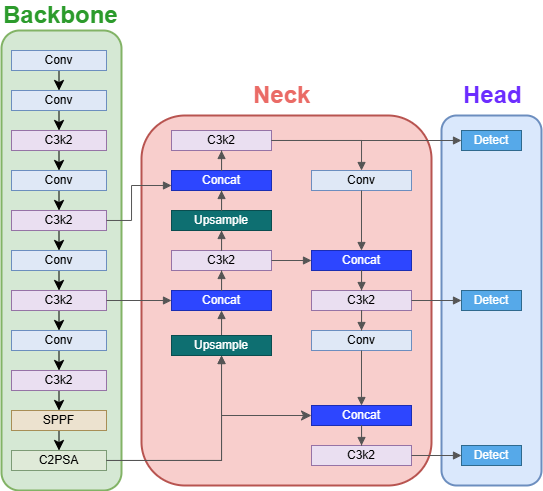
\includegraphics[width=0.8\linewidth]{images/yolo11.drawio.png}
    \caption{Simplified overview of the YOLO11 architecture, showing the backbone, neck, and head structure.}
    \label{fig:yolo11_architecture}
\end{figure}


A major theme in modern YOLO development is that improvements are typically introduced through refinements to internal building blocks rather than through complete architectural redesign. Across recent versions, this has included lighter feature extraction modules, improved multi-scale pooling, and the increasing use of attention mechanisms to strengthen global context modelling. In parallel, head design has also evolved toward more efficient and deployment-oriented inference, with newer models seeking to reduce computational overhead while maintaining strong detection performance. As a result, recent YOLO models can be understood as sharing a common single-stage detection framework while differing in how they optimize feature extraction, attention, training strategy, and inference efficiency \cite{UltralyticsYOLO}.

\subsubsection{YOLO11 Architecture}

YOLO11 retains the standard modern YOLO backbone--neck--head pipeline, but introduces several architectural refinements relative to earlier Ultralytics versions. Its backbone begins with two stride-2 convolutional layers, after which the main feature extraction stages are built around the \textit{C3k2} block rather than the \textit{C2f} block used in earlier models such as YOLOv8. The reviewed paper describes C3k2 as a lighter and more advanced replacement intended to reduce parameter count while preserving strong representational capacity. It also notes that the internal behaviour of C3k2 depends on variant, with larger YOLO11 models consistently using the \textit{C3k} path. This makes YOLO11 an example of the broader trend toward improving efficiency through more carefully designed internal modules rather than major changes to the overall detector layout \cite{UltralyticsYOLO}.

After the backbone, YOLO11 applies \textit{SPPF} and then \textit{C2PSA} before entering the main neck fusion pathway. SPPF provides multi-scale pooling, while C2PSA introduces a self-attention mechanism to improve global feature modelling. Importantly, the attention block is placed only at the lowest-resolution stage in order to limit computational cost. The neck then uses repeated upsampling and concatenation operations to merge deep semantic features with higher-resolution features from earlier backbone stages, before passing them to a three-scale detection head for small, medium, and large object detection. Overall, YOLO11 preserves the established multi-scale YOLO framework, but distinguishes itself through the use of C3k2, C2PSA, and related lightweight convolutional refinements that improve efficiency without fundamentally altering the architecture \cite{UltralyticsYOLO}.

\subsubsection{YOLO26 Architecture}

YOLO26 is architecturally very similar to YOLO11 and preserves the same overall backbone, neck, and head structure, including the use of stride-2 convolutions in the stem, \textit{C3k2} blocks for feature extraction, \textit{SPPF} and \textit{C2PSA} near the bottleneck, and a three-scale detection head \cite{UltralyticsYOLO}. However, the literature describes YOLO26 as an incremental refinement of YOLO11 rather than a direct continuation without change. One architectural modification is the addition of a shortcut connection inside the \textit{SPPF} block, which is intended to improve information flow and stabilize optimization at high semantic levels. A second change is in the final \textit{C3k2} block before detection, where YOLO26 incorporates an attention mechanism through a \textit{PSABlock}, aiming to strengthen global context modelling without a large increase in parameters or latency \cite{UltralyticsYOLO}.

The more substantial differences between YOLO26 and YOLO11 occur in the detection and training pipeline. The paper states that YOLO26 removes \textit{Distribution Focal Loss (DFL)} from the detect block and instead uses direct box regression, simplifying both training and inference. It also adopts a dual-assignment, end-to-end, NMS-free design inspired by YOLOv10, where one-to-many and one-to-one assignments are both used during training, but only the one-to-one path is retained at inference. In addition, YOLO26 introduces \textit{Progressive Loss Balancing (ProgLoss)} and \textit{Small-Target-Aware Label Assignment (STAL)} to improve training stability and enhance learning for small objects, alongside the \textit{MuSGD} optimizer for smoother convergence. Consequently, while YOLO26 looks very similar to YOLO11 at the high level, it differs in several important architectural and training details that push it further toward edge-oriented, end-to-end, and small-object-aware detection \cite{UltralyticsYOLO}.

\subsection{Literature Review: Compression Techniques}

A range of model compression techniques designed to reduce the computational and memory requirements of deep learning models (while preserving acceptable analytical performance) have been explored in literature. Although these techniques have not yet been widely applied to end-to-end football statistic generation systems, they will form a strong foundation for deploying real-time soccer analysis pipelines on edge devices.


\subsubsection{Efficiency Techniques: Hardware Acceleration}

Hardware acceleration improves inference efficiency by executing neural networks through runtimes and software stacks that are specifically optimized for the target hardware platform \cite{tensorrt}. Rather than relying on a default framework execution path, accelerated backends can apply graph-level optimizations, fuse operations, select more efficient kernels, and better exploit GPU parallelism. This is particularly important in real-time computer vision, where inference latency directly affects whether a system can operate at interactive or live processing speeds.

A common approach to hardware acceleration in embedded and GPU-based deep learning systems is the use of optimized inference runtimes such as TensorRT. These frameworks convert trained models into deployment-ready representations that are tailored to the hardware on which inference will be performed. By moving much of the optimization work offline, such approaches reduce runtime overhead and improve throughput, making them especially valuable in edge settings where compute and power budgets are constrained.

\begin{figure}[H]
    \centering
    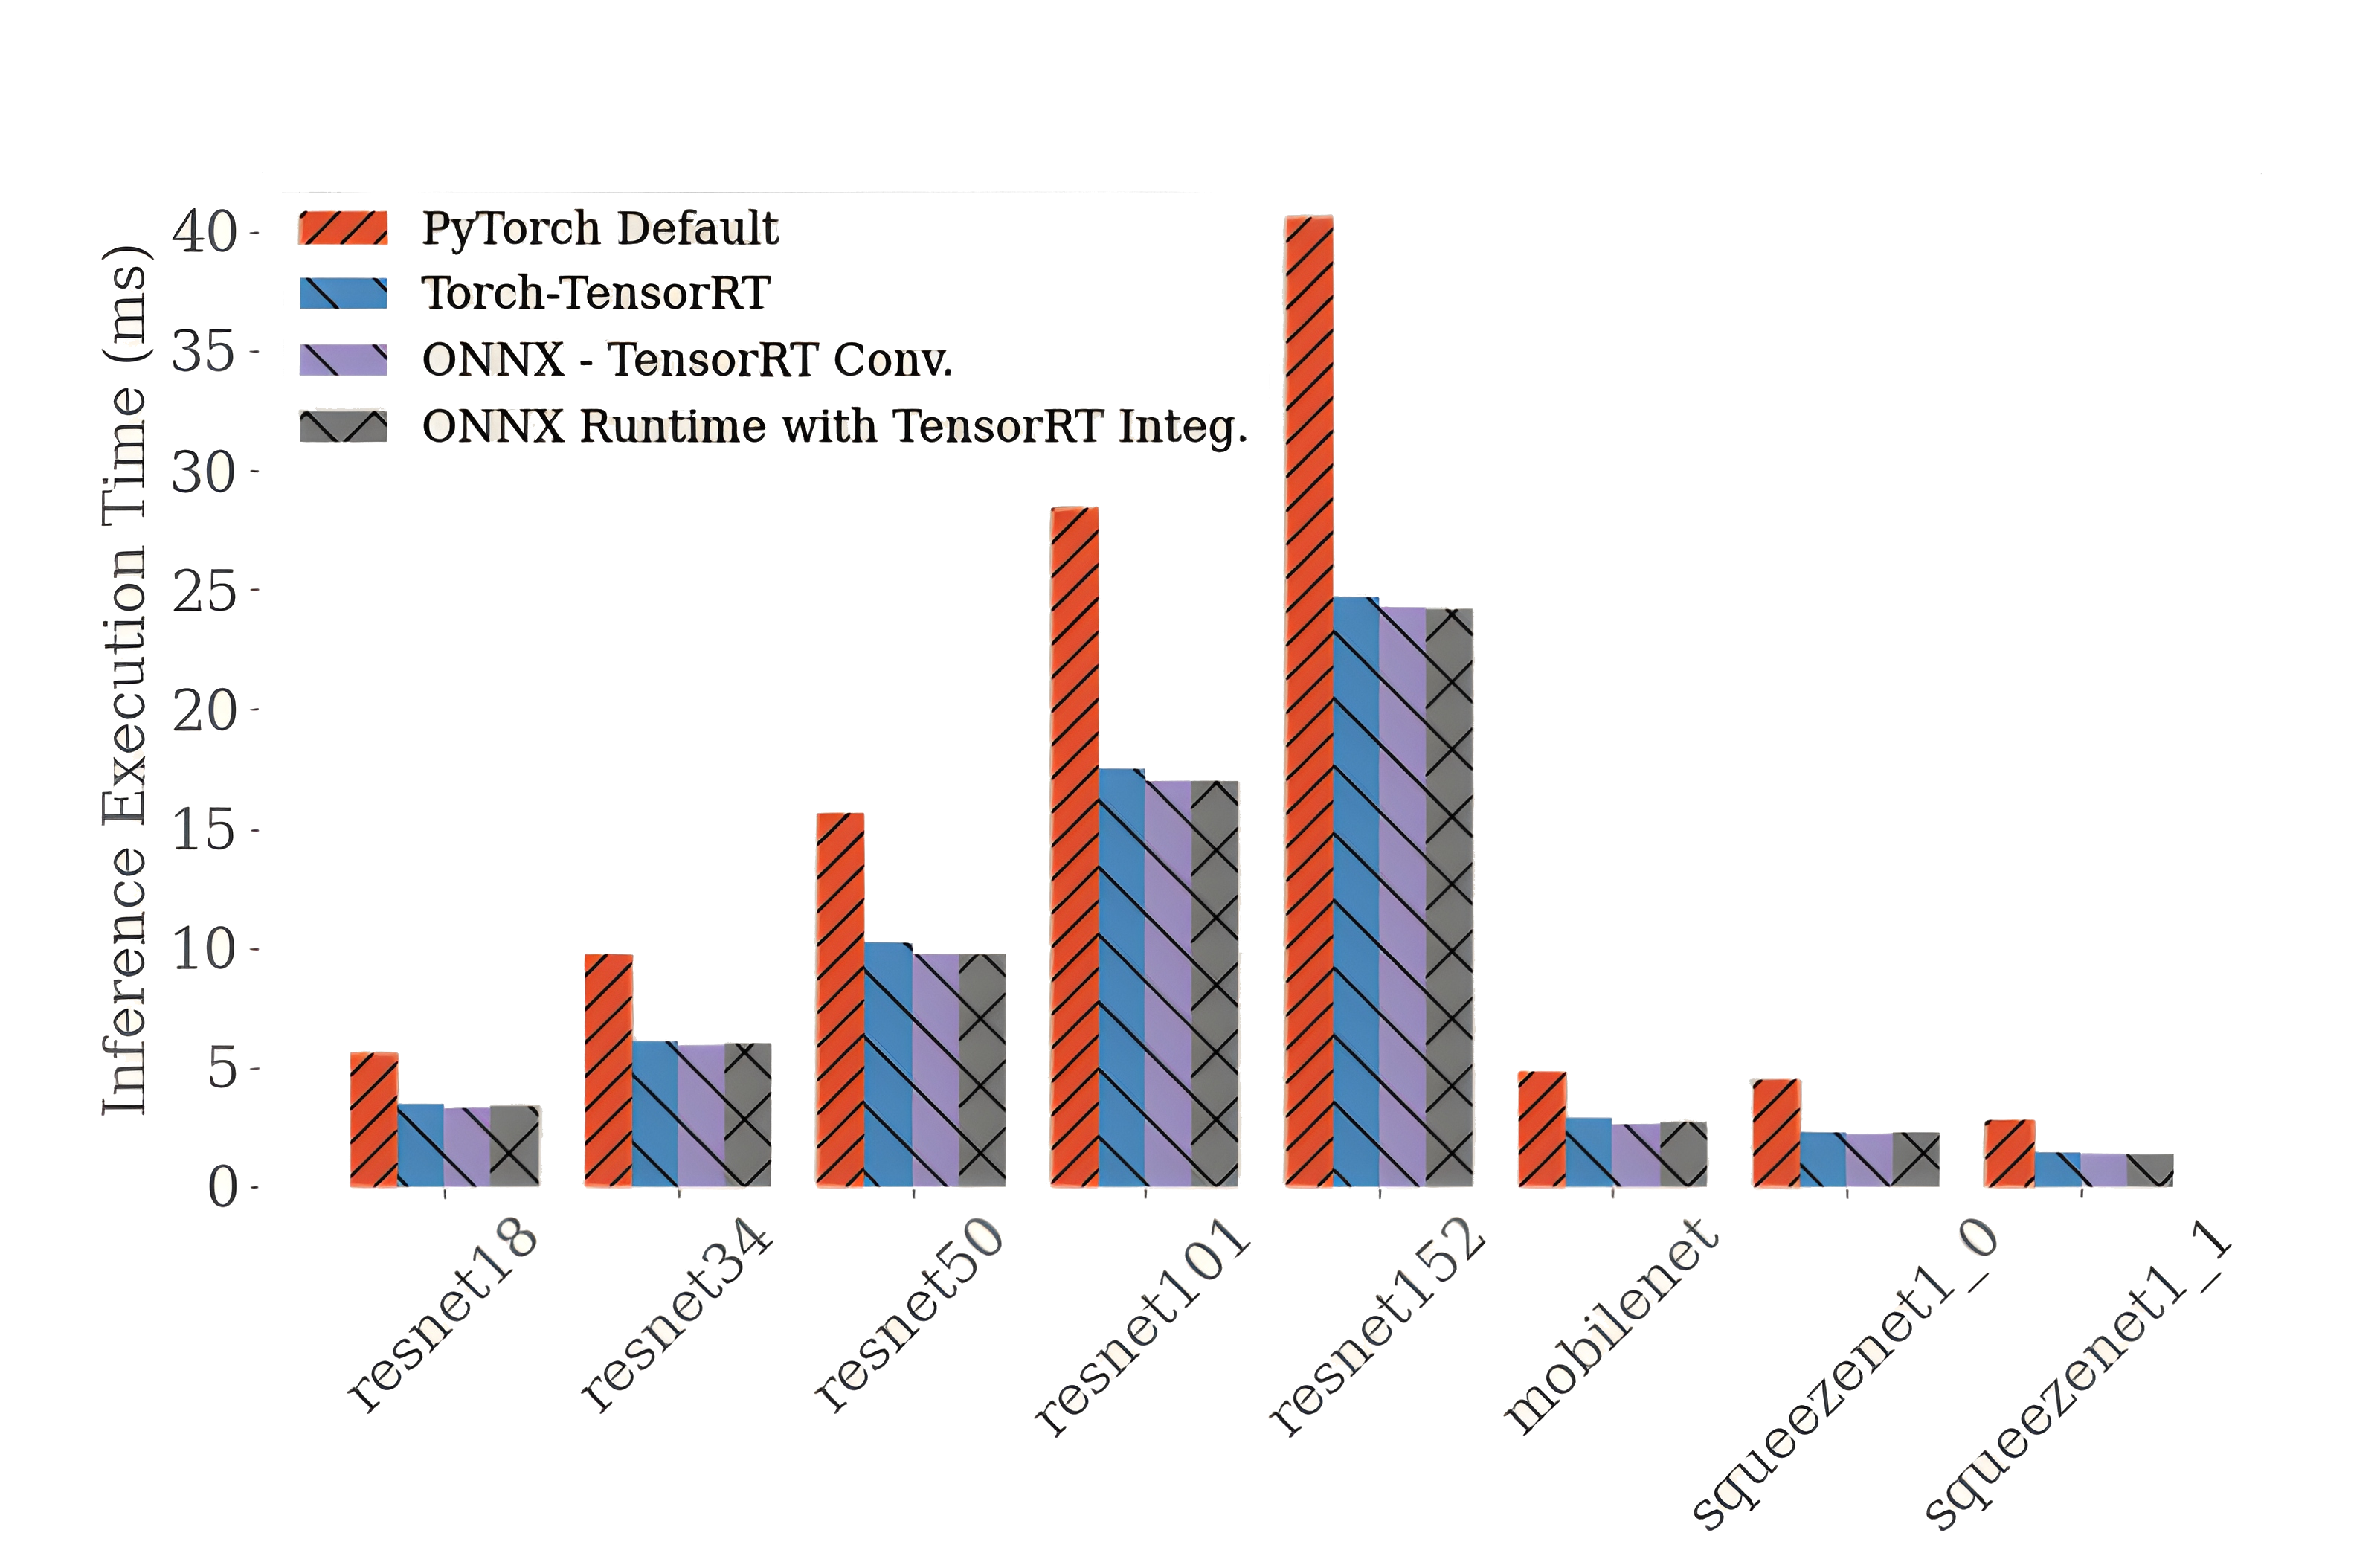
\includegraphics[width=0.6\linewidth]{images/628b6d9a-fb26-4df1-bafa-aab8cca775f1.png}
    \caption{Effect of \texttt{tensorrt} application on inference time.}
    \label{fig:hardware_acceleration_lit}
\end{figure}

Figure~\ref{fig:hardware_acceleration_lit} illustrates the typical effect of hardware acceleration on inference execution time \cite{tensorrt}. As can be seen, optimized TensorRT-based pipelines consistently reduce latency relative to the default PyTorch implementation, with similar trends also observed for ONNX-based accelerated deployment. This demonstrates that hardware acceleration can provide substantial efficiency improvements without altering the underlying model task, making it an important optimization strategy in the deployment of real-time computer vision systems.


\subsubsection{Compression Techniques: Quantization}

Quantization is one of the most widely adopted compression techniques, and involves reducing the numerical precision of model parameters and activations \cite{inbook}. While standard, uncompressed neural networks typically utilise 32-bit floating-point (FP32) representations, quantization maps these values to lower-precision formats such as 8-bit (INT8) or 4-bit (INT4) integers.  This process substantially reduces memory bandwidth usage and arithmetic complexity, with INT8 addition being up to 30× more energy-efficient and 116× more area-efficient than its FP32 counterpart on 45nm hardware \cite{inbook}. Figure \ref{fig:quantlit} below displays the effect of different quantization levels on device power consumption.

\begin{figure}[H]
    \centering
    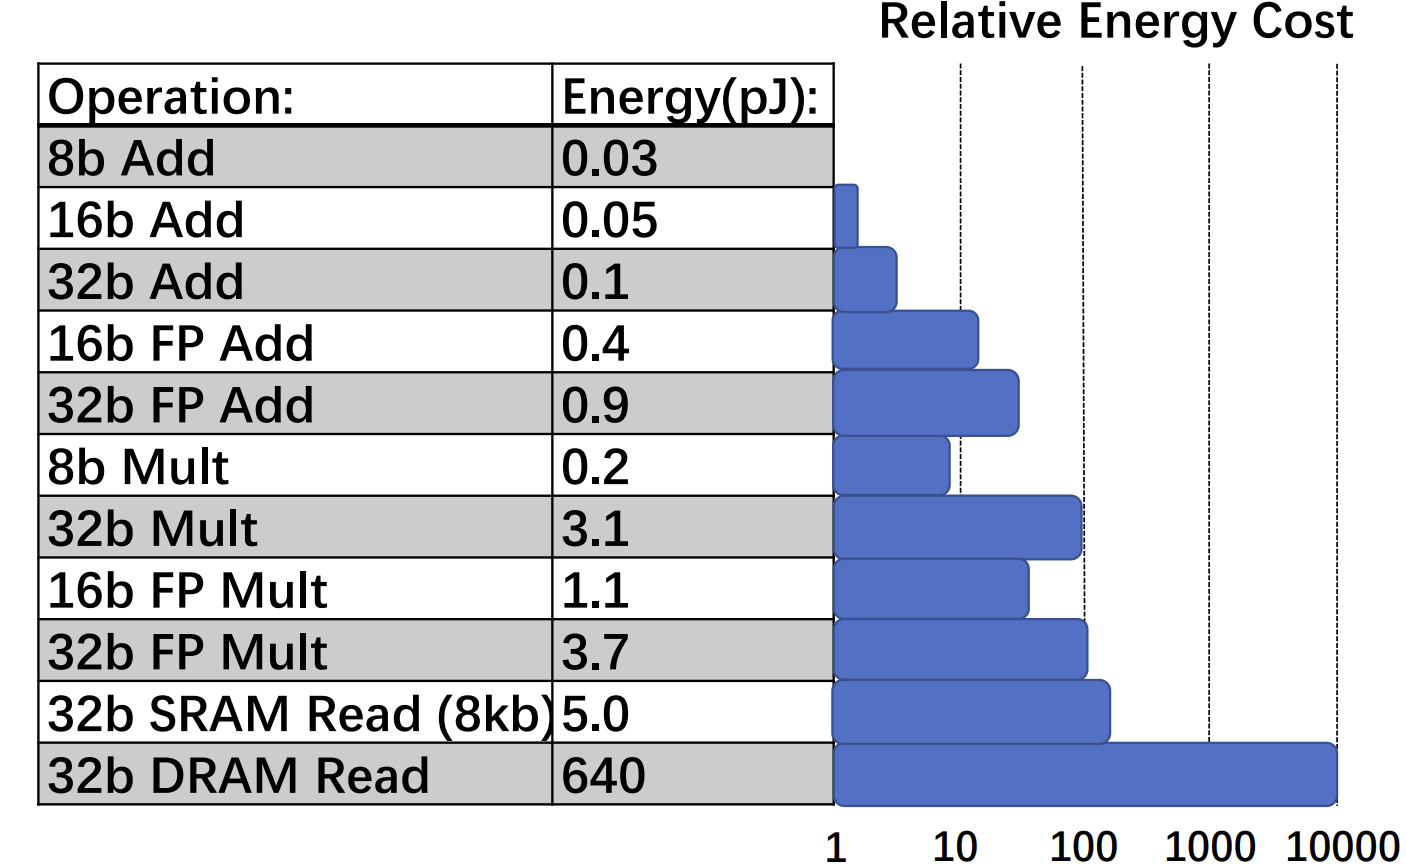
\includegraphics[width=0.5\linewidth]{images/quantization.png}
    \caption{Effect of Quantization of Model Energy Consumption \cite{inbook}}
    \label{fig:quantlit}
\end{figure}

As can be seen, identical operations utilise significantly less energy (in Joules) when using less precise values. For example, an 8-bit multiplication requires 0.2 pJ, while a 32b multiplication requires 3.1 pJ. This demonstrates the clear optimization benefit that quantization can supply.

\subsubsection{Compression Techniques: Pruning}

The technique of pruning aims to reduce model complexity by removing parameters that contribute minimally to the network’s output \cite{inbook, 10204354}. This technique follows the assumption that the smallest system capable of fitting the training data typically yields the best generalization on unseen inputs \cite{248452}. It is often performed after training, where a loss function is used to estimate the importance of weights, before identifying and eliminating redundant connections. 

Pruning strategies are fundamentally divided into unstructured and structured approaches. Unstructured pruning removes individual weights with low importance regardless of their location \cite{inbook}, which achieves high compression ratios at the cost of efficient memory manipulation. Structured pruning removes whole structures such as entire filters, channels, or layers, which maintains efficient memory at the cost of less compression. \cite{10204354}. Figure \ref{fig:pruninglit} below displays model accuracy (TOP-1) and FLOPS, when various pruning strategies are applied.

\begin{figure}[H]
    \centering
    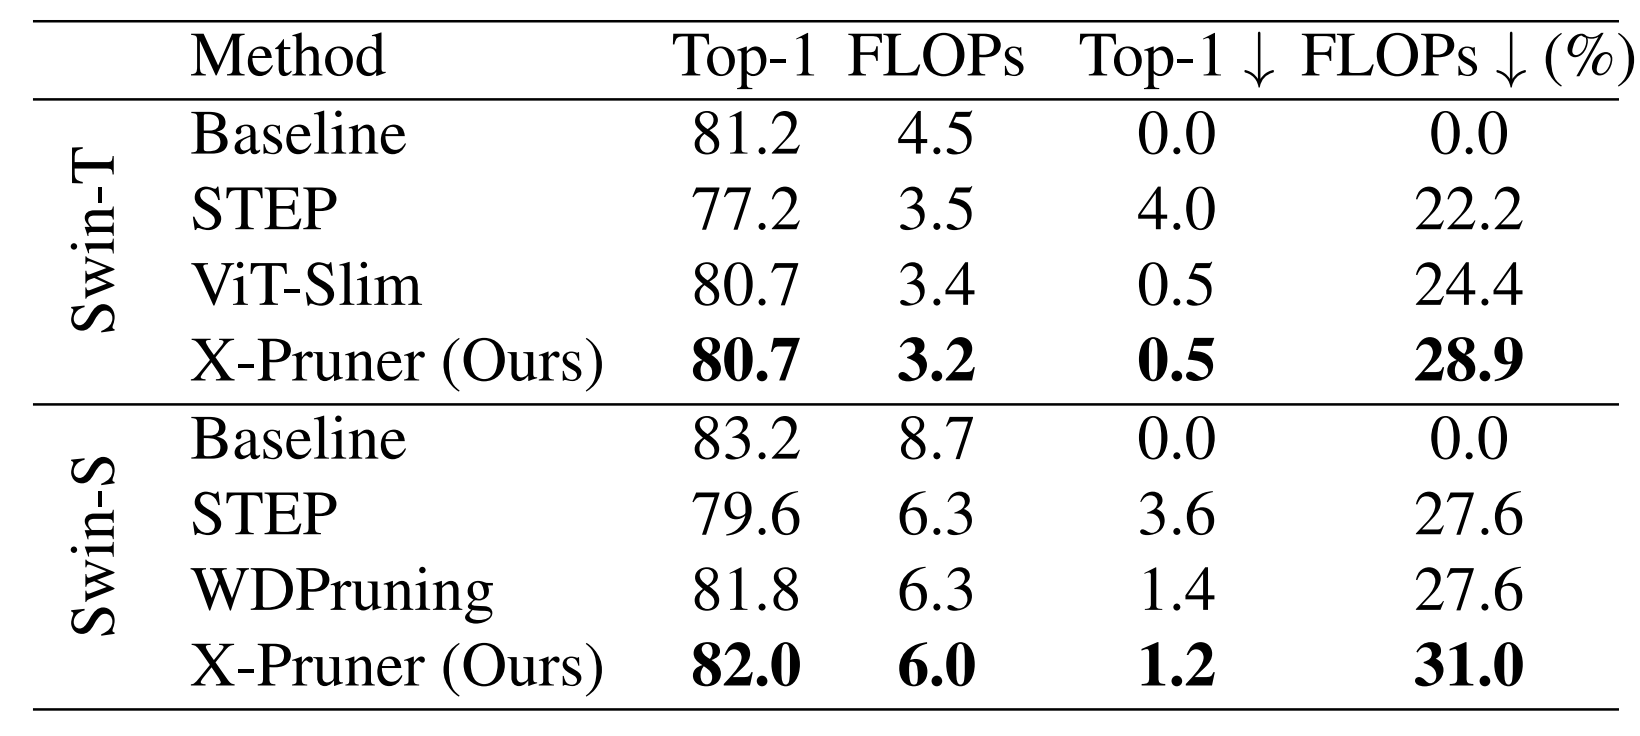
\includegraphics[width=0.6\linewidth]{images/pruning.png}
    \caption{Effect of Pruning on Accuracy and FLOPS \cite{10204354}}
    \label{fig:pruninglit}
\end{figure}

As can be seen, applying the X-Pruner algorithm reduces the required FLOPS by 28\%, with only a .5\% reduction in accuracy (Top-1). For this reason, pruning will be explored as a method of compressing training soccer computer vision models. 

\subsubsection{Compression Techniques: Input Resolution Scaling}
Input resolution scaling reduces computational and memory footprints by lowering the spatial dimensions of the images or tokens processed by a model. Since the complexity of Convolutional Neural Networks and Vision Transformers typically scales quadratically with input resolution, even modest downsizing can yield substantial improvements in inference throughput and energy efficiency \cite{morlier2025input}. Figure \ref{fig:inputreslit} displays model characteristics (FLOPS and memory usage) before and after input resolution scaling is applied. 

\begin{figure}[H]
    \centering
    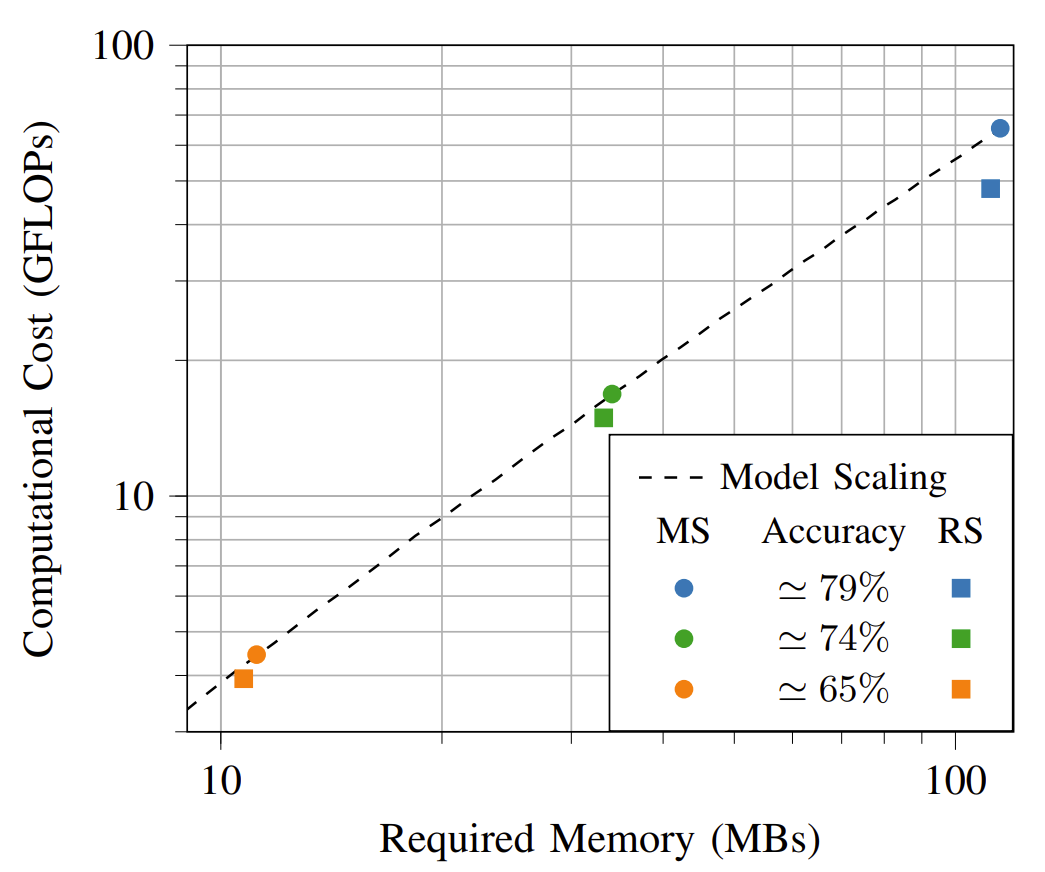
\includegraphics[width=0.6\linewidth]{images/inputresresearch.png}
    \caption{Required Memory Vs. FLOPS when Input Resolution Scaling is Applied \cite{morlier2025input}}
    \label{fig:inputreslit}
\end{figure}


As can be seen by Figure \ref{fig:inputreslit}, applying input resolution scaling often reduces the required FLOPS by $\sim$2x, with slight improvements in required memory. However, this technique may introduce a major accuracy/efficiency trade-off, as reducing resolution compromises the detection of small objects \cite{morlier2025input, zheng2025_review_football_cv}. In the soccer domain, where the ball often occupies fewer than 100 pixels, resolution is a primary determinant of performance; for instance, increasing resolution from 640px to 1200px has been shown to improve ball detection recall by up to 96\% \cite{10756443}. To mitigate these losses, implementations often utilise training-evaluation discrepancies, training models on smaller resized crops but evaluating at slightly higher resolutions to recover analytical performance \cite{morlier2025input}.

\subsubsection{Compression Techniques: Knowledge Distillation}
Knowledge distillation is another model compression technique, in which a compact "student" model is trained to replicate the performance of a high-capacity "teacher" model. Unlike standard training, the student is optimised using softened output distributions (logits) or intermediate feature representations produced by the teacher, which contain richer information than hard ground-truth labels \cite{Kaleem2024ACR, inbook}. Knowledge transfer can be categorised into three types: response-based, which focuses on the final output probabilities; feature-based, which aims to mimic the teacher's internal feature maps to capture implicit patterns; and relation-based, which teaches the student the relationships between different data samples or layers \cite{Kaleem2024ACR}. 
